%%%%%%%%%%%%%%%%%%%%%%%%%%%%%%%%%%%%%%%%%
% University/School Laboratory Report
% LaTeX Template
% Version 2.0 (4/12/12)
%
% This template has been downloaded from:
% http://www.latextemplates.com
%
% License:
% CC BY-NC-SA 3.0 (http://creativecommons.org/licenses/by-nc-sa/3.0/)
%
% Original header:
%
% This is a LaTeX version of the sample laboratory report
% from Virginia Tech's copyrighted 08-09 CHEM 1045/1046 lab manual.
% Reproduction of this one appendix section for academic purposes
% should fall under fair use.
%
%%%%%%%%%%%%%%%%%%%%%%%%%%%%%%%%%%%%%%%%%

\documentclass{article}
\usepackage{graphicx}
\usepackage{mathtools}

\title{ELEC 302-81\\ Lab 1\\ Power in AC Circuits} % Title
% \author{John \textsc{Smith}} % Author name
\date{\today} % Specify a date for the report

\begin{document}

\maketitle

\begin{center}
  \begin{tabular}{l r}
    Date Performed: & January 14, 2013 \\
    Partners: & Rawley Dent \\
    & Charles Pittman \\
    Instructor: & Dr. Weatherford
  \end{tabular}
\end{center}

\pagebreak

\setlength\parindent{0pt} % Removes all indentation from paragraphs

\section{Purpose of Experiment}
In this experiment, an RLC circuit was modeled on an EMS workstation.
The capacitance was varied for two different inductance values. The circuit
was then analyzed to obtain measured values for the circuit power factor, real
power, and apparent power. These measured results were then compared to the 
theoretical values calculated beforehand. Familiarization with the EMS
workstaton was also obtained.

\section{Circuit Tested}
\begin{figure}[h]
  \begin{center}
    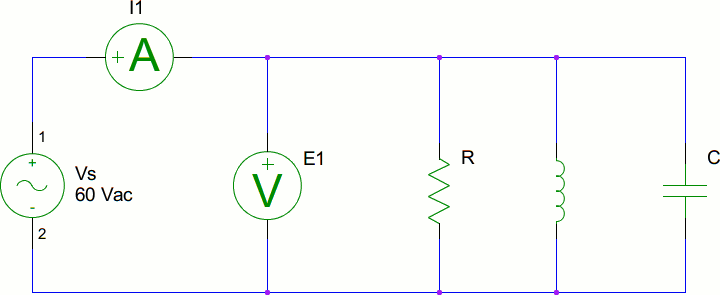
\includegraphics[width=.8\textwidth]{test_circuit}
    \caption{Parallel RLC Circuit Configuration}
    \label{test_circuit}
  \end{center}
\end{figure}

\begin{table}[h]
  \begin{center}
    \begin{tabular}{ccc}
      \hline
      R & L & C \\
      $\Omega$ & H & $\mu$F \\
      \hline
      1200 & 0.8 & --- \\ 1200 & 0.8 & 2.2 \\ 1200 & 0.8 & 4.4 \\
      1200 & 0.8 & 8.8 \\ 1200 & 1.6 & --- \\ 1200 & 1.6 & 2.2 \\
      1200 & 1.6 & 4.4 \\ 1200 & 1.6 & 8.8 \\
      \hline
    \end{tabular}
    \caption{RLC Values for circuit in Figure~\ref{test_circuit}}
    \label{testc_dat}
  \end{center}
\end{table}

\section{Procedure}
At the EMS workstation, the main power switch of the Power Supply was 
verified to be OFF, and the voltage control knob was verified to be 
completely counterclockwise. The voltmeter selector switch was set to
position 4-N. The RLC circuit shown in Figure 1 was modeled with the 
capacitor left out at first. The elements labeled E1 and I1 on Figure 1
refered to the ammeter and voltmeter Data Acquisition Interface (DAI)
connections. The DAI 24-V supply was connected to the main Power Supply,
and the DAI USB cable was connected to the PC workstation. The main power
switch of the Power Supply was switched to ON.

On the PC, the Lab-Volt Data Acquisition Management application was
started, and the file pertaining to the experiment being worked was 
opened. Three windows (metering, oscilloscope, and phasor analyzer)
were verified to open up along with the experiment file. The three 
windows were set to continuously refresh.

The supply voltage was adjusted to read 24-V. Verification was obtained
by monitoring the EMS analog voltmeter and the digital metering window
on the PC. The load voltage E1, load current I1, the real power consumed 
by the circuit, and the phase angle were recorded. In the Phasor Analyzer
window, E1 was selected as the reference phasor. The voltage control knob 
was then turn completely counterclockwise and the main power switch was 
set to OFF.

The EMS workstation was then reconfigured to include the capacitance.
The subsequent values included in Table 3 were then measured.

\section{Calc}
\begin{table}[h]
  \begin{center}
    \begin{tabular}{cccccccccc}
      \hline
      R & L & C & I$_1$ & E$_1$ & P & $\theta$ & S & Q & p.f. \\
      $\Omega$ & H & $\mu$F & A & V & W & $\circ$ & VA & VAR & \\
      \hline
      1200 & 0.8 & --- & 0.210 & 60 & 4.56 &  68.77 & 12.58 & 11.73 & 0.36 \\
      1200 & 0.8 & 2.2 & 0.164 & 60 & 4.56 &  62.48 &  9.86 &  8.75 & 0.46 \\
      1200 & 0.8 & 4.4 & 0.122 & 60 & 4.56 &  51.65 &  7.34 &  5.76 & 0.62 \\
      1200 & 0.8 & 8.8 & 0.076 & 60 & 4.56 &  -2.67 &  4.56 & -0.21 & 1.00 \\
      1200 & 1.6 & --- & 0.114 & 60 & 3.39 &  60.27 &  6.84 &  5.94 & 0.50 \\
      1200 & 1.6 & 2.2 & 0.075 & 60 & 3.39 &  41.06 &  4.50 &  2.96 & 0.75 \\
      1200 & 1.6 & 4.4 & 0.057 & 60 & 3.39 &  -0.50 &  3.39 & -0.03 & 1.00 \\
      1200 & 1.6 & 8.8 & 0.115 & 60 & 3.39 & -60.51 &  6.89 & -6.00 & 0.49 \\
      \hline
    \end{tabular}
    \caption{Calculated Data}
    \label{calc_dat}
  \end{center}
\end{table}

\[\mathbf{P} = \mathbf{VI}\cos\theta \]
\[\mathbf{Q} = \mathbf{VI}\sin\theta\]
\[\mathbf{S} = \mathbf{VI}^*\]
\[\mathbf{V} = \mathbf{IZ}\]
\[\text{p.f.} = \cos\theta\]

\section{Results}
\begin{table}[h]
  \begin{center}
    \begin{tabular}{cccccccccc}
      \hline
      R & L & C & I$_1$ & E$_1$ & P & $\theta$ & S & Q & p.f. \\
      $\Omega$ & H & $\mu$F & A & V & W & $\circ$ & VA & VAR & \\
      \hline
      1200 & 0.8 & --- & 0.206 & 60.9 & 4.53 &  68.0 & 12.55 & 11.21 & 0.37 \\
      1200 & 0.8 & 2.2 & 0.158 & 60.9 & 4.56 &  60.9 &  9.62 &  8.19 & 0.49 \\
      1200 & 0.8 & 4.4 & 0.117 & 60.9 & 4.59 &  49.0 &  7.13 &  5.28 & 0.66 \\
      1200 & 0.8 & 8.8 & 0.081 & 61.0 & 4.65 &  -4.4 &  4.94 & -0.36 & 1.00 \\
      1200 & 1.6 & --- & 0.116 & 61.0 & 3.94 &  55.4 &  7.08 &  0.37 & 1.00 \\
      1200 & 1.6 & 2.2 & 0.079 & 61.0 & 3.96 &  32.8 &  4.82 &  2.55 & 0.84 \\
      1200 & 1.6 & 4.4 & 0.067 & 61.0 & 3.99 &  -6.6 &  4.09 & -0.46 & 1.00 \\
      1200 & 1.6 & 8.8 & 0.124 & 61.2 & 4.05 & -57.4 &  7.60 & -6.33 & 0.54 \\
      \hline
    \end{tabular}
    \caption{Experimental Data}
    \label{meas_dat}
  \end{center}
\end{table}

\section{Comparison with Theoretical: Percent Deviation}
\begin{table}[h]
  \begin{center}
    \begin{tabular}{cccccccccc}
      \hline
      R & L & C & I$_1$ & E$_1$ & P & $\theta$ & S & Q & p.f. \\
      \hline
      0.0 & 0.0 & --- & 1.9 & 1.5 & 0.7 & 1.1 & 0.2 & 4.4 & 2.8 \\
      0.0 & 0.0 & 0.0 & 3.7 & 1.5 & 0.0 & 2.5 & 2.4 & 6.4 & 6.5 \\
      0.0 & 0.0 & 0.0 & 4.1 & 1.5 & 0.7 & 5.1 & 2.9 & 8.3 & 6.5 \\
      0.0 & 0.0 & 0.0 & 6.6 & 1.7 & 2.0 & 65  & 8.3 & 71  & 0.0 \\
      0.0 & 0.0 & --- & 1.8 & 1.7 & 16  & 8.1 & 3.5 & 94  & 100 \\
      0.0 & 0.0 & 0.0 & 5.3 & 1.7 & 17  & 20  & 7.1 & 14  & 12  \\
      0.0 & 0.0 & 0.0 & 18  & 1.7 & 18  & 1220& 21  & 1433& 0.0 \\
      0.0 & 0.0 & 0.0 & 7.8 & 2.0 & 19  & 5.1 & 10  & 5.5 & 10  \\

\[\text{\%deviation} = \frac{measured - theoretical}{theoretical}\ \times \text{100\%}\]

\section{Conclusions}
The effects of different levels of capacitance were observed by 
conducting this experiemnt. The theoretical values for real power, 
apparent power, and the phase angle were calculated. Then, 
the experiment was conducted to verify the effects of a parallel 
RLC circuit. These measured results were differed from the theoretical
results because of one underlying reason. The switch modeling the 
inductance at the EMS workstation contained an internal impedance.
This added impedance caused the calculted results to differ from the 
measured. Also, one can see that the voltage measured at E1 fluctuating throughout
the experiment. This fluctuation caused added variations between measured
and theoretical. 

It was noted that row 8 of Tables 2 and 3 contained a negative angle for
the phase impedance. This signified a highly capacitative load where the phase 
current lead the phase voltage. All other loads were inductive, except in
rows 4 and 7, where the load was slightly capacitative. In these rows, 4 and
7, the power factor recorded as 1.0 signifiying an inuctive load efficiently 
corrected by a capacitance.

\end{document}
